\documentclass[tikz,border=2pt]{standalone}
\usepackage{amsmath}
\usetikzlibrary{arrows.meta}
\begin{document}
% Work in the system between two arrivals (A = (1,2,5,9,10), S = (3,2,1,2,2)).
% Left: W_2 = 2, S_2 = 2, X_3 = 3, so W_3 = [2+2-3]^+ = 1. Right: W_3 = 1, S_3 = 1, X_4 = 4,
% the work hits zero at t = 7 and the server idles until t = 9, so W_4 = [1+1-4]^+ = 0.
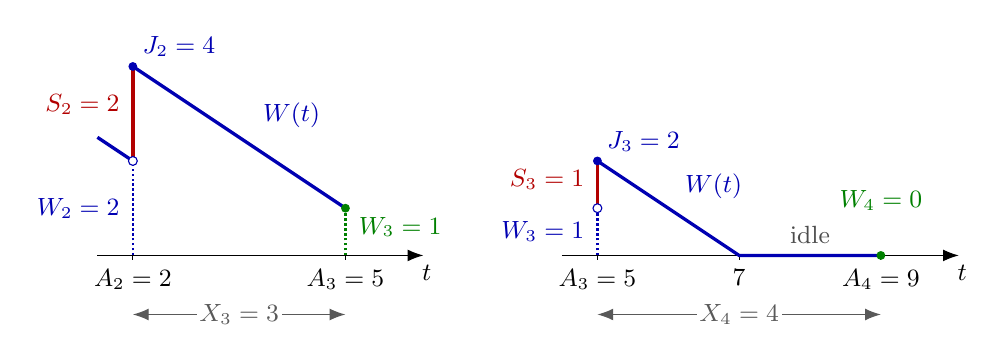
\begin{tikzpicture}[font=\small, >={Latex[length=2mm]}, x=0.9cm, y=0.6cm]
  % ---------- left panel: t = 1.5 ... 5.3, u = t - 1.5
  \begin{scope}
    \draw[->] (0,0) -- (4.6,0) node[anchor=north west, xshift=-4pt] {$t$};
    \node[blue!70!black, anchor=south west] at (2.2,2.5) {$W(t)$};
    \foreach \u/\lab in {0.5/{A_2=2}, 3.5/{A_3=5}} \draw (\u,0) -- (\u,-0.1) node[below] {$\lab$};
    \draw[<->, gray!70!black] (0.5,-1.25) -- node[fill=white, inner sep=1pt] {$X_3=3$} (3.5,-1.25);
    \draw[blue!70!black, very thick] (0,2.5) -- (0.5,2);
    \draw[blue!70!black, thick, densely dotted] (0.5,0) -- (0.5,2);
    \draw[red!70!black, very thick] (0.5,2) -- (0.5,4);
    \draw[blue!70!black, very thick] (0.5,4) -- (3.5,1);
    \draw[green!50!black, thick, densely dotted] (3.5,0) -- (3.5,1);
    \draw[blue!70!black, fill=white] (0.5,2) circle (1.6pt);
    \fill[blue!70!black] (0.5,4) circle (1.6pt);
    \fill[green!50!black] (3.5,1) circle (1.6pt);
    \node[blue!70!black, anchor=east] at (0.45,1) {$W_2=2$};
    \node[red!70!black, anchor=east] at (0.45,3.2) {$S_2=2$};
    \node[blue!70!black, anchor=south west] at (0.5,4) {$J_2=4$};
    \node[green!50!black, anchor=west] at (3.55,0.6) {$W_3=1$};
  \end{scope}
  % ---------- right panel: t = 4.5 ... 9.8, u = t - 4.5
  \begin{scope}[xshift=5.9cm]
    \draw[->] (0,0) -- (5.6,0) node[anchor=north west, xshift=-4pt] {$t$};
    \node[blue!70!black, anchor=south west] at (1.6,1.0) {$W(t)$};
    \foreach \u/\lab in {0.5/{A_3=5}, 2.5/{7}, 4.5/{A_4=9}} \draw (\u,0) -- (\u,-0.1) node[below] {$\lab$};
    \draw[<->, gray!70!black] (0.5,-1.25) -- node[fill=white, inner sep=1pt] {$X_4=4$} (4.5,-1.25);
    \draw[blue!70!black, thick, densely dotted] (0.5,0) -- (0.5,1);
    \draw[red!70!black, very thick] (0.5,1) -- (0.5,2);
    \draw[blue!70!black, very thick] (0.5,2) -- (2.5,0) -- (4.5,0);
    \draw[blue!70!black, fill=white] (0.5,1) circle (1.6pt);
    \fill[blue!70!black] (0.5,2) circle (1.6pt);
    \fill[green!50!black] (4.5,0) circle (1.6pt);
    \node[blue!70!black, anchor=east] at (0.45,0.5) {$W_3=1$};
    \node[red!70!black, anchor=east] at (0.45,1.6) {$S_3=1$};
    \node[blue!70!black, anchor=south west] at (0.5,2) {$J_3=2$};
    \node[gray!60!black, anchor=south] at (3.5,0.05) {idle};
    \node[green!50!black, anchor=south] at (4.5,0.75) {$W_4=0$};
  \end{scope}
\end{tikzpicture}
\end{document}
